\documentclass[twoside]{book}

% Packages required by doxygen
\usepackage{calc}
\usepackage{doxygen}
\usepackage{graphicx}
\usepackage[utf8]{inputenc}
\usepackage{makeidx}
\usepackage{multicol}
\usepackage{multirow}
\usepackage{textcomp}
\usepackage[table]{xcolor}

% NLS support packages
Portuguese
% Font selection
\usepackage[T1]{fontenc}
\usepackage{mathptmx}
\usepackage[scaled=.90]{helvet}
\usepackage{courier}
\usepackage{amssymb}
\usepackage{sectsty}
\renewcommand{\familydefault}{\sfdefault}
\allsectionsfont{%
  \fontseries{bc}\selectfont%
  \color{darkgray}%
}
\renewcommand{\DoxyLabelFont}{%
  \fontseries{bc}\selectfont%
  \color{darkgray}%
}

% Page & text layout
\usepackage{geometry}
\geometry{%
  a4paper,%
  top=2.5cm,%
  bottom=2.5cm,%
  left=2.5cm,%
  right=2.5cm%
}
\tolerance=750
\hfuzz=15pt
\hbadness=750
\setlength{\emergencystretch}{15pt}
\setlength{\parindent}{0cm}
\setlength{\parskip}{0.2cm}
\makeatletter
\renewcommand{\paragraph}{%
  \@startsection{paragraph}{4}{0ex}{-1.0ex}{1.0ex}{%
    \normalfont\normalsize\bfseries\SS@parafont%
  }%
}
\renewcommand{\subparagraph}{%
  \@startsection{subparagraph}{5}{0ex}{-1.0ex}{1.0ex}{%
    \normalfont\normalsize\bfseries\SS@subparafont%
  }%
}
\makeatother

% Headers & footers
\usepackage{fancyhdr}
\pagestyle{fancyplain}
\fancyhead[LE]{\fancyplain{}{\bfseries\thepage}}
\fancyhead[CE]{\fancyplain{}{}}
\fancyhead[RE]{\fancyplain{}{\bfseries\leftmark}}
\fancyhead[LO]{\fancyplain{}{\bfseries\rightmark}}
\fancyhead[CO]{\fancyplain{}{}}
\fancyhead[RO]{\fancyplain{}{\bfseries\thepage}}
\fancyfoot[LE]{\fancyplain{}{}}
\fancyfoot[CE]{\fancyplain{}{}}
\fancyfoot[RE]{\fancyplain{}{\bfseries\scriptsize Gerado em Terça, 15 de Maio de 2018 16\-:30\-:49 para Lab 3 Lojinha por Doxygen }}
\fancyfoot[LO]{\fancyplain{}{\bfseries\scriptsize Gerado em Terça, 15 de Maio de 2018 16\-:30\-:49 para Lab 3 Lojinha por Doxygen }}
\fancyfoot[CO]{\fancyplain{}{}}
\fancyfoot[RO]{\fancyplain{}{}}
\renewcommand{\footrulewidth}{0.4pt}
\renewcommand{\chaptermark}[1]{%
  \markboth{#1}{}%
}
\renewcommand{\sectionmark}[1]{%
  \markright{\thesection\ #1}%
}

% Indices & bibliography
\usepackage{natbib}
\usepackage[titles]{tocloft}
\setcounter{tocdepth}{3}
\setcounter{secnumdepth}{5}
\makeindex

% Hyperlinks (required, but should be loaded last)
\usepackage{ifpdf}
\ifpdf
  \usepackage[pdftex,pagebackref=true]{hyperref}
\else
  \usepackage[ps2pdf,pagebackref=true]{hyperref}
\fi
\hypersetup{%
  colorlinks=true,%
  linkcolor=blue,%
  citecolor=blue,%
  unicode%
}

% Custom commands
\newcommand{\clearemptydoublepage}{%
  \newpage{\pagestyle{empty}\cleardoublepage}%
}


%===== C O N T E N T S =====

\begin{document}

% Titlepage & ToC
\hypersetup{pageanchor=false}
\pagenumbering{roman}
\begin{titlepage}
\vspace*{7cm}
\begin{center}%
{\Large Lab 3 Lojinha \\[1ex]\large Programa que simula uma loja de conveniência }\\
\vspace*{1cm}
{\large Gerado por Doxygen 1.8.6}\\
\vspace*{0.5cm}
{\small Terça, 15 de Maio de 2018 16:30:49}\\
\end{center}
\end{titlepage}
\clearemptydoublepage
\tableofcontents
\clearemptydoublepage
\pagenumbering{arabic}
\hypersetup{pageanchor=true}

%--- Begin generated contents ---
\chapter{R\-E\-A\-D\-M\-E}
\label{d0/d30/md_README}
\hypertarget{d0/d30/md_README}{}
\section*{M\-E\-N\-S\-A\-G\-E\-M D\-O T\-E\-O\-B\-A\-L\-D\-O}

\subparagraph*{}

Caro amigo, nem sei por onde começar. Soube do desastre que foi a avaliação, mas eu realmente tive que viajar e não deu tempo de completar as implementações.

A propósito, acabo de notar que estou atrasado para outra viagem...

Hey! Posso te pedir mais um G\-R\-A\-N\-D\-E favor? Completa esse código para mim?!

Não se esqueça de\-:
\begin{DoxyItemize}
\item Completar a implementação das classes
\item Documentar o código usando Doxygen
\item Criar um makefile apropiado
\item Alterar o main para testar toda a implementação
\end{DoxyItemize}

I\-M\-P\-O\-R\-T\-A\-N\-T\-E\-:
\begin{DoxyItemize}
\item Não permita incluir na lista produtos com o mesmo código
\item Confesso que apenas reproduzi a sobrecarga do operador de inserção na classe \hyperlink{classProduto}{Produto}, mas não sei bem o que fiz. O que eu realmente não entendi foi como, mesmo eu não tendo sobrecarregado o operador de inserção na classe \hyperlink{classFruta}{Fruta}, ainda consigo imprimir os dados de um objeto desta classe usando este operador! Que loucura! Por isso, preciso que você explique isso em um ou dois parágrafos para eu enviar ao professor.
\item Outra parte que eu fiz, mas não sei bem a razão, foi declarar o método destrutor da classe \hyperlink{classProduto}{Produto} como virtual. Advinha?! Eu também preciso explicar isso ao professor. Conto com sua ajuda!
\end{DoxyItemize}

Fico te devendo mais esta!

Tenho que ir.

Teobaldo 
\chapter{Índice da hierarquia}
\section{Hierarquia de classes}
Esta lista de heranças está organizada, dentro do possível, por ordem alfabética\-:\begin{DoxyCompactList}
\item \contentsline{section}{Produto}{\pageref{d8/d30/classProduto}}{}
\begin{DoxyCompactList}
\item \contentsline{section}{Bebida}{\pageref{df/de2/classBebida}}{}
\item \contentsline{section}{Fruta}{\pageref{d4/d5f/classFruta}}{}
\item \contentsline{section}{Roupa}{\pageref{d9/d53/classRoupa}}{}
\end{DoxyCompactList}
\end{DoxyCompactList}

\chapter{Índice dos componentes}
\section{Lista de componentes}
Lista de classes, estruturas, uniões e interfaces com uma breve descrição\-:\begin{DoxyCompactList}
\item\contentsline{section}{\hyperlink{classBebida}{Bebida} \\*Classe \hyperlink{classBebida}{Bebida}, derivada de \hyperlink{classProduto}{Produto} }{\pageref{df/de2/classBebida}}{}
\item\contentsline{section}{\hyperlink{classFruta}{Fruta} \\*Classe \hyperlink{classFruta}{Fruta}, derivada de \hyperlink{classProduto}{Produto} }{\pageref{d4/d5f/classFruta}}{}
\item\contentsline{section}{\hyperlink{classProduto}{Produto} }{\pageref{d8/d30/classProduto}}{}
\item\contentsline{section}{\hyperlink{classRoupa}{Roupa} \\*Classe \hyperlink{classRoupa}{Roupa}, derivada de \hyperlink{classProduto}{Produto} }{\pageref{d9/d53/classRoupa}}{}
\end{DoxyCompactList}

\chapter{Índice dos ficheiros}
\section{Lista de ficheiros}
Lista de todos os ficheiros documentados com uma breve descrição\-:\begin{DoxyCompactList}
\item\contentsline{section}{{\bfseries roupa.\-h} }{\pageref{d3/d06/roupa_8h}}{}
\item\contentsline{section}{include/\hyperlink{bebida_8h}{bebida.\-h} \\*Definição da classe \hyperlink{classBebida}{Bebida} em C++ }{\pageref{d7/daf/bebida_8h}}{}
\item\contentsline{section}{include/\hyperlink{fruta_8h}{fruta.\-h} \\*Definição da classe \hyperlink{classFruta}{Fruta} em C++ }{\pageref{dc/d4a/fruta_8h}}{}
\item\contentsline{section}{include/\hyperlink{produto_8h}{produto.\-h} \\*Definição da classe \hyperlink{classProduto}{Produto} em C++ }{\pageref{d2/de5/produto_8h}}{}
\item\contentsline{section}{include/{\bfseries roupa.\-h} }{\pageref{d2/d60/include_2roupa_8h}}{}
\item\contentsline{section}{src/\hyperlink{bebida_8cpp}{bebida.\-cpp} \\*Implementação da classe \hyperlink{classBebida}{Bebida} em C++ }{\pageref{da/d8e/bebida_8cpp}}{}
\item\contentsline{section}{src/\hyperlink{fruta_8cpp}{fruta.\-cpp} \\*Implementação da classe \hyperlink{classFruta}{Fruta} em C++ }{\pageref{d5/d5f/fruta_8cpp}}{}
\item\contentsline{section}{src/\hyperlink{produto_8cpp}{produto.\-cpp} \\*Implementação da classe \hyperlink{classProduto}{Produto} em C++ }{\pageref{d1/d04/produto_8cpp}}{}
\item\contentsline{section}{src/\hyperlink{roupa_8cpp}{roupa.\-cpp} \\*Implementação da classe \hyperlink{classRoupa}{Roupa} em C++ }{\pageref{da/dbd/roupa_8cpp}}{}
\end{DoxyCompactList}

\chapter{Documentação da classe}
\hypertarget{classBebida}{\section{Referência à classe Bebida}
\label{classBebida}\index{Bebida@{Bebida}}
}


Classe \hyperlink{classBebida}{Bebida}, derivada de \hyperlink{classProduto}{Produto}.  




{\ttfamily \#include $<$bebida.\-h$>$}

Diagrama de heranças da classe Bebida\begin{figure}[H]
\begin{center}
\leavevmode
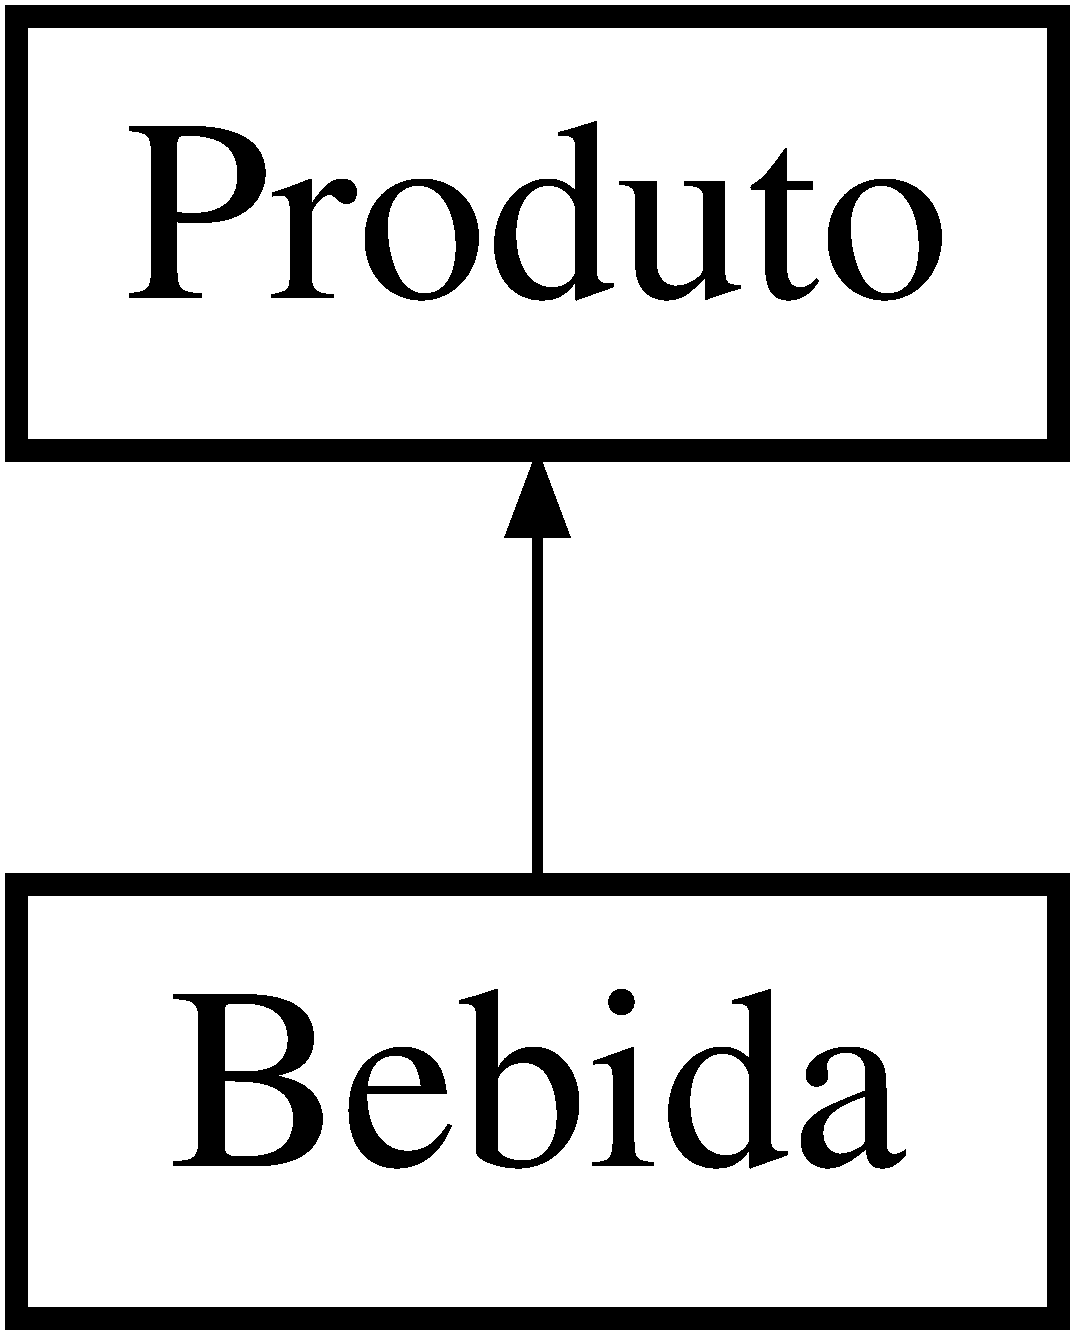
\includegraphics[height=2.000000cm]{df/de2/classBebida}
\end{center}
\end{figure}
\subsection*{Membros públicos}
\begin{DoxyCompactItemize}
\item 
\hypertarget{classBebida_afab3bc3b54a7e55049ed36fae3479dfb}{\hyperlink{classBebida_afab3bc3b54a7e55049ed36fae3479dfb}{Bebida} ()}\label{classBebida_afab3bc3b54a7e55049ed36fae3479dfb}

\begin{DoxyCompactList}\small\item\em Método construtor padrão de \hyperlink{classBebida}{Bebida}. \end{DoxyCompactList}\item 
\hyperlink{classBebida_a4f8e4f45e2b42c62591193127c7c0ea5}{Bebida} (int \hyperlink{classProduto_a76711f92305c825f07549734cd7c6ade}{tag}, string codigo\-Barra, string \hyperlink{classProduto_ab04a024e24feb7f79774e280356f6bc7}{descricao}, short \hyperlink{classProduto_a2ad13f91582fd70e878fc449c7b77171}{preco}, short teor\-Alcoolico)
\begin{DoxyCompactList}\small\item\em Método construtor parametrizado de \hyperlink{classBebida}{Bebida}. \end{DoxyCompactList}\item 
\hypertarget{classBebida_a4ed0a8b2b0b464f2b39ef81a01e297ad}{\hyperlink{classBebida_a4ed0a8b2b0b464f2b39ef81a01e297ad}{$\sim$\-Bebida} ()}\label{classBebida_a4ed0a8b2b0b464f2b39ef81a01e297ad}

\begin{DoxyCompactList}\small\item\em Interface destrutor de \hyperlink{classProduto}{Produto} definida para \hyperlink{classBebida}{Bebida}  Método virtual da classe \hyperlink{classProduto}{Produto} redefinida para um objeto \hyperlink{classBebida}{Bebida}. \end{DoxyCompactList}\item 
short \hyperlink{classBebida_a12416f60ae201da672ab9cd950d2fa70}{get\-Teor\-Alcoolico} ()
\begin{DoxyCompactList}\small\item\em Método de captura do teor\-Alcoolico. \end{DoxyCompactList}\item 
void \hyperlink{classBebida_afa75fe87caa8ede5d41edfb0dab031f2}{set\-Teor\-Alcoolico} (short teor\-Alcoolico)
\begin{DoxyCompactList}\small\item\em Método de atribuição de teor\-Alcoolico. \end{DoxyCompactList}\end{DoxyCompactItemize}
\subsection*{Additional Inherited Members}


\subsection{Descrição detalhada}
Classe \hyperlink{classBebida}{Bebida}, derivada de \hyperlink{classProduto}{Produto}. 

\subsection{Documentação dos Construtores \& Destrutor}
\hypertarget{classBebida_a4f8e4f45e2b42c62591193127c7c0ea5}{\index{Bebida@{Bebida}!Bebida@{Bebida}}
\index{Bebida@{Bebida}!Bebida@{Bebida}}
\subsubsection[{Bebida}]{\setlength{\rightskip}{0pt plus 5cm}Bebida\-::\-Bebida (
\begin{DoxyParamCaption}
\item[{int}]{tag, }
\item[{string}]{codigo\-Barra, }
\item[{string}]{descricao, }
\item[{short}]{preco, }
\item[{short}]{teor\-Alcoolico}
\end{DoxyParamCaption}
)}}\label{classBebida_a4f8e4f45e2b42c62591193127c7c0ea5}


Método construtor parametrizado de \hyperlink{classBebida}{Bebida}. 


\begin{DoxyParams}{Parâmetros}
{\em int} & tag -\/ categoria do \hyperlink{classProduto}{Produto} \\
\hline
{\em string} & codigo -\/ Codigo de barras do \hyperlink{classProduto}{Produto} \\
\hline
{\em string} & descricao -\/ Descrição do \hyperlink{classProduto}{Produto} \\
\hline
{\em short} & preco -\/ Preço do \hyperlink{classProduto}{Produto} \\
\hline
{\em short} & teor\-Alcoolico -\/ Descrição da porcentagem do teor alcoolico da bebida\\
\hline
\end{DoxyParams}
$<$ inicialização da classe base \hyperlink{classProduto}{Produto} 

\subsection{Documentação dos métodos}
\hypertarget{classBebida_a12416f60ae201da672ab9cd950d2fa70}{\index{Bebida@{Bebida}!get\-Teor\-Alcoolico@{get\-Teor\-Alcoolico}}
\index{get\-Teor\-Alcoolico@{get\-Teor\-Alcoolico}!Bebida@{Bebida}}
\subsubsection[{get\-Teor\-Alcoolico}]{\setlength{\rightskip}{0pt plus 5cm}short Bebida\-::get\-Teor\-Alcoolico (
\begin{DoxyParamCaption}
{}
\end{DoxyParamCaption}
)}}\label{classBebida_a12416f60ae201da672ab9cd950d2fa70}


Método de captura do teor\-Alcoolico. 

\begin{DoxyReturn}{Retorna}
Retorna a porcentagem do teor alcoolico da bebida 
\end{DoxyReturn}
\hypertarget{classBebida_afa75fe87caa8ede5d41edfb0dab031f2}{\index{Bebida@{Bebida}!set\-Teor\-Alcoolico@{set\-Teor\-Alcoolico}}
\index{set\-Teor\-Alcoolico@{set\-Teor\-Alcoolico}!Bebida@{Bebida}}
\subsubsection[{set\-Teor\-Alcoolico}]{\setlength{\rightskip}{0pt plus 5cm}void Bebida\-::set\-Teor\-Alcoolico (
\begin{DoxyParamCaption}
\item[{short}]{teor\-Alcoolico}
\end{DoxyParamCaption}
)}}\label{classBebida_afa75fe87caa8ede5d41edfb0dab031f2}


Método de atribuição de teor\-Alcoolico. 


\begin{DoxyParams}{Parâmetros}
{\em Recebe} & string teor\-Alcoolico \\
\hline
\end{DoxyParams}


A documentação para esta classe foi gerada a partir dos seguintes ficheiros\-:\begin{DoxyCompactItemize}
\item 
include/\hyperlink{bebida_8h}{bebida.\-h}\item 
src/\hyperlink{bebida_8cpp}{bebida.\-cpp}\end{DoxyCompactItemize}

\hypertarget{classFruta}{\section{Referência à classe Fruta}
\label{classFruta}\index{Fruta@{Fruta}}
}


Classe \hyperlink{classFruta}{Fruta}, derivada de \hyperlink{classProduto}{Produto}.  




{\ttfamily \#include $<$fruta.\-h$>$}

Diagrama de heranças da classe Fruta\begin{figure}[H]
\begin{center}
\leavevmode
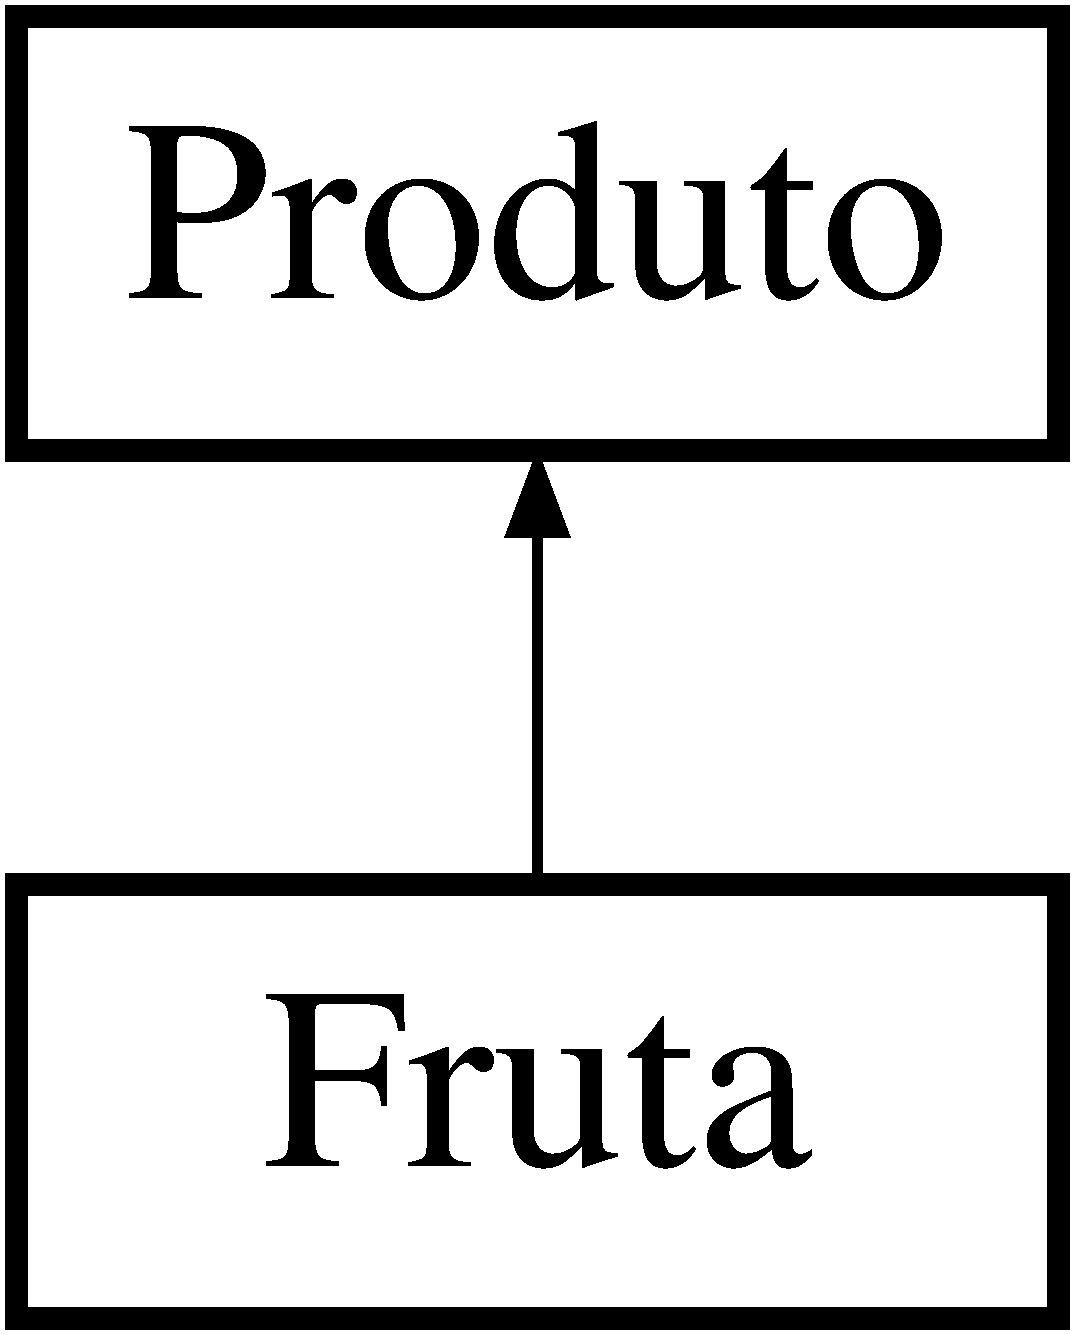
\includegraphics[height=2.000000cm]{d4/d5f/classFruta}
\end{center}
\end{figure}
\subsection*{Membros públicos}
\begin{DoxyCompactItemize}
\item 
\hypertarget{classFruta_ae1b52e5f60e121e940e9523e71b38e2d}{\hyperlink{classFruta_ae1b52e5f60e121e940e9523e71b38e2d}{Fruta} ()}\label{classFruta_ae1b52e5f60e121e940e9523e71b38e2d}

\begin{DoxyCompactList}\small\item\em Método construtor padrão de \hyperlink{classFruta}{Fruta}. \end{DoxyCompactList}\item 
\hyperlink{classFruta_aac6c8cb8aaf52d5da49d136f574f0fbc}{Fruta} (int \hyperlink{classProduto_a76711f92305c825f07549734cd7c6ade}{tag}, std\-::string codigo, std\-::string \hyperlink{classProduto_ab04a024e24feb7f79774e280356f6bc7}{descricao}, short \hyperlink{classProduto_a2ad13f91582fd70e878fc449c7b77171}{preco}, std\-::string data, short validade)
\begin{DoxyCompactList}\small\item\em Método construtor parametrizado de \hyperlink{classFruta}{Fruta}. \end{DoxyCompactList}\item 
\hypertarget{classFruta_a634920474b757127cb86443d402f84dd}{\hyperlink{classFruta_a634920474b757127cb86443d402f84dd}{$\sim$\-Fruta} ()}\label{classFruta_a634920474b757127cb86443d402f84dd}

\begin{DoxyCompactList}\small\item\em Interface destrutor de \hyperlink{classProduto}{Produto} definida para \hyperlink{classFruta}{Fruta}  Método virtual da classe \hyperlink{classProduto}{Produto} redefinida para um objeto \hyperlink{classFruta}{Fruta}. \end{DoxyCompactList}\item 
std\-::string \hyperlink{classFruta_a89525ef74d892639b1a56dbf1c6ffe61}{get\-Data\-Lote} ()
\begin{DoxyCompactList}\small\item\em Método de captura de data\-\_\-lote. \end{DoxyCompactList}\item 
short \hyperlink{classFruta_ab12db1faf3d5a0743ab461bc3315832e}{get\-Validade} ()
\begin{DoxyCompactList}\small\item\em Método de captura de validade. \end{DoxyCompactList}\item 
void \hyperlink{classFruta_a9aa6275d0da3c9c80430bce35a3d0467}{set\-Data\-Lote} (std\-::string data)
\begin{DoxyCompactList}\small\item\em Método de atribuição de data\-\_\-lote. \end{DoxyCompactList}\item 
void \hyperlink{classFruta_a0ea71bcde4ec328dcfcad0b377848bef}{set\-Validade} (short validade)
\begin{DoxyCompactList}\small\item\em Método de atribuição de validade. \end{DoxyCompactList}\end{DoxyCompactItemize}
\subsection*{Additional Inherited Members}


\subsection{Descrição detalhada}
Classe \hyperlink{classFruta}{Fruta}, derivada de \hyperlink{classProduto}{Produto}. 

\subsection{Documentação dos Construtores \& Destrutor}
\hypertarget{classFruta_aac6c8cb8aaf52d5da49d136f574f0fbc}{\index{Fruta@{Fruta}!Fruta@{Fruta}}
\index{Fruta@{Fruta}!Fruta@{Fruta}}
\subsubsection[{Fruta}]{\setlength{\rightskip}{0pt plus 5cm}Fruta\-::\-Fruta (
\begin{DoxyParamCaption}
\item[{int}]{tag, }
\item[{std\-::string}]{codigo\-Barra, }
\item[{std\-::string}]{descricao, }
\item[{short}]{preco, }
\item[{std\-::string}]{data, }
\item[{short}]{validade}
\end{DoxyParamCaption}
)}}\label{classFruta_aac6c8cb8aaf52d5da49d136f574f0fbc}


Método construtor parametrizado de \hyperlink{classFruta}{Fruta}. 


\begin{DoxyParams}{Parâmetros}
{\em int} & tag -\/ categoria do \hyperlink{classProduto}{Produto} \\
\hline
{\em string} & codigo -\/ Codigo de barras do \hyperlink{classProduto}{Produto} \\
\hline
{\em string} & descricao -\/ Descrição do \hyperlink{classProduto}{Produto} \\
\hline
{\em short} & preco -\/ Preço do \hyperlink{classProduto}{Produto} \\
\hline
{\em string} & data -\/ Define a data do lote da fruta \\
\hline
{\em short} & validade -\/ Define os dias para vencimento a partir da data do lote\\
\hline
\end{DoxyParams}
inicialização da classe base \hyperlink{classProduto}{Produto} 

\subsection{Documentação dos métodos}
\hypertarget{classFruta_a89525ef74d892639b1a56dbf1c6ffe61}{\index{Fruta@{Fruta}!get\-Data\-Lote@{get\-Data\-Lote}}
\index{get\-Data\-Lote@{get\-Data\-Lote}!Fruta@{Fruta}}
\subsubsection[{get\-Data\-Lote}]{\setlength{\rightskip}{0pt plus 5cm}std\-::string Fruta\-::get\-Data\-Lote (
\begin{DoxyParamCaption}
{}
\end{DoxyParamCaption}
)}}\label{classFruta_a89525ef74d892639b1a56dbf1c6ffe61}


Método de captura de data\-\_\-lote. 

\begin{DoxyReturn}{Retorna}
Retorna a data de lote do produto 
\end{DoxyReturn}
\hypertarget{classFruta_ab12db1faf3d5a0743ab461bc3315832e}{\index{Fruta@{Fruta}!get\-Validade@{get\-Validade}}
\index{get\-Validade@{get\-Validade}!Fruta@{Fruta}}
\subsubsection[{get\-Validade}]{\setlength{\rightskip}{0pt plus 5cm}short Fruta\-::get\-Validade (
\begin{DoxyParamCaption}
{}
\end{DoxyParamCaption}
)}}\label{classFruta_ab12db1faf3d5a0743ab461bc3315832e}


Método de captura de validade. 

\begin{DoxyReturn}{Retorna}
Retorna a validade 
\end{DoxyReturn}
\hypertarget{classFruta_a9aa6275d0da3c9c80430bce35a3d0467}{\index{Fruta@{Fruta}!set\-Data\-Lote@{set\-Data\-Lote}}
\index{set\-Data\-Lote@{set\-Data\-Lote}!Fruta@{Fruta}}
\subsubsection[{set\-Data\-Lote}]{\setlength{\rightskip}{0pt plus 5cm}void Fruta\-::set\-Data\-Lote (
\begin{DoxyParamCaption}
\item[{std\-::string}]{data}
\end{DoxyParamCaption}
)}}\label{classFruta_a9aa6275d0da3c9c80430bce35a3d0467}


Método de atribuição de data\-\_\-lote. 


\begin{DoxyParams}{Parâmetros}
{\em Recebe} & string data \\
\hline
\end{DoxyParams}
\hypertarget{classFruta_a0ea71bcde4ec328dcfcad0b377848bef}{\index{Fruta@{Fruta}!set\-Validade@{set\-Validade}}
\index{set\-Validade@{set\-Validade}!Fruta@{Fruta}}
\subsubsection[{set\-Validade}]{\setlength{\rightskip}{0pt plus 5cm}void Fruta\-::set\-Validade (
\begin{DoxyParamCaption}
\item[{short}]{validade}
\end{DoxyParamCaption}
)}}\label{classFruta_a0ea71bcde4ec328dcfcad0b377848bef}


Método de atribuição de validade. 


\begin{DoxyParams}{Parâmetros}
{\em Recebe} & string validade \\
\hline
\end{DoxyParams}


A documentação para esta classe foi gerada a partir dos seguintes ficheiros\-:\begin{DoxyCompactItemize}
\item 
include/\hyperlink{fruta_8h}{fruta.\-h}\item 
src/\hyperlink{fruta_8cpp}{fruta.\-cpp}\end{DoxyCompactItemize}

\hypertarget{classProduto}{\section{Referência à classe Produto}
\label{classProduto}\index{Produto@{Produto}}
}
Diagrama de heranças da classe Produto\begin{figure}[H]
\begin{center}
\leavevmode
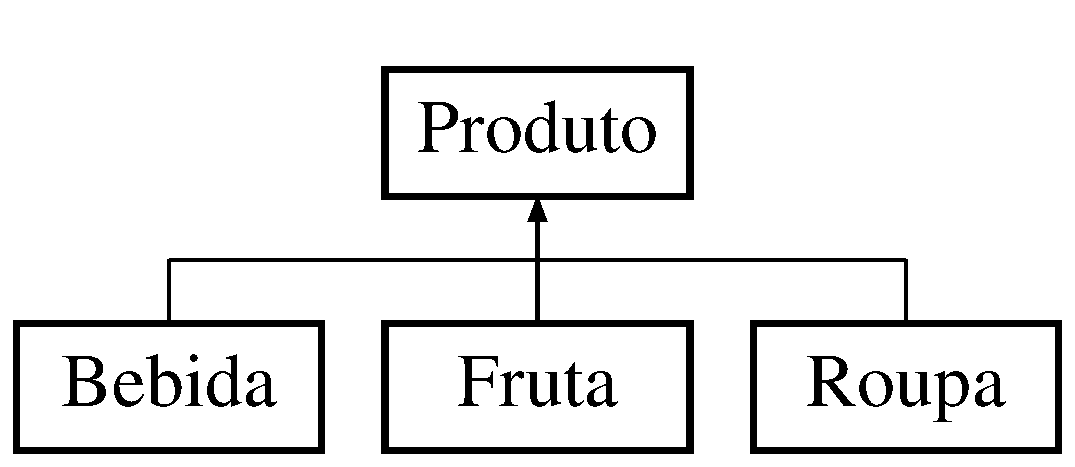
\includegraphics[height=2.000000cm]{d8/d30/classProduto}
\end{center}
\end{figure}
\subsection*{Membros públicos}
\begin{DoxyCompactItemize}
\item 
\hypertarget{classProduto_adcd5834a1f04cc42fef88bf60217b8f4}{\hyperlink{classProduto_adcd5834a1f04cc42fef88bf60217b8f4}{Produto} ()}\label{classProduto_adcd5834a1f04cc42fef88bf60217b8f4}

\begin{DoxyCompactList}\small\item\em Método construtor padrão de produto. \end{DoxyCompactList}\item 
\hyperlink{classProduto_ae44d64ad61a5fa8b0f7af193a2f526f4}{Produto} (int \hyperlink{classProduto_a76711f92305c825f07549734cd7c6ade}{tag}, std\-::string codigo, std\-::string \hyperlink{classProduto_ab04a024e24feb7f79774e280356f6bc7}{descricao}, short \hyperlink{classProduto_a2ad13f91582fd70e878fc449c7b77171}{preco})
\begin{DoxyCompactList}\small\item\em Método construtor parametrizado de produto. \end{DoxyCompactList}\item 
\hypertarget{classProduto_a84a8b28176b743e8c74bfd89aee9a9b2}{virtual \hyperlink{classProduto_a84a8b28176b743e8c74bfd89aee9a9b2}{$\sim$\-Produto} ()}\label{classProduto_a84a8b28176b743e8c74bfd89aee9a9b2}

\begin{DoxyCompactList}\small\item\em Interface destrutor de \hyperlink{classProduto}{Produto}  Método virtual da classe \hyperlink{classProduto}{Produto} capaz de ser redefinido (sobrecarregado) por suas classes derivadas. \end{DoxyCompactList}\item 
int \hyperlink{classProduto_a60c26b830a7fd5409a7b4e5a3abcecce}{get\-Tag} ()
\begin{DoxyCompactList}\small\item\em Método de captura da Tag. \end{DoxyCompactList}\item 
std\-::string \hyperlink{classProduto_aa8e9057d5f0ac3d145333223cb513b3e}{get\-Cod\-Barras} ()
\begin{DoxyCompactList}\small\item\em Método de captura de Cod\-Barras. \end{DoxyCompactList}\item 
std\-::string \hyperlink{classProduto_ada2c72e139e09afa967aa06a4290d5f8}{get\-Descricao} ()
\begin{DoxyCompactList}\small\item\em Método de captura de Descrição. \end{DoxyCompactList}\item 
double \hyperlink{classProduto_a53548783d7fad3ea6d5e000fa2227dcf}{get\-Preco} ()
\begin{DoxyCompactList}\small\item\em Método de captura de preço. \end{DoxyCompactList}\item 
void \hyperlink{classProduto_adec0c5a9864579405d522f0d405396d9}{set\-Cod\-Barras} (std\-::string codigo)
\begin{DoxyCompactList}\small\item\em Método de atribuição de Cod\-Barras. \end{DoxyCompactList}\item 
void \hyperlink{classProduto_afdc63d61e7948b1ae4b72b29d1115571}{set\-Descricao} (std\-::string \hyperlink{classProduto_ab04a024e24feb7f79774e280356f6bc7}{descricao})
\begin{DoxyCompactList}\small\item\em Método de atribuição de Descrição. \end{DoxyCompactList}\item 
void \hyperlink{classProduto_aba1d39de900f61e612219a42781f7f7e}{set\-Preco} (double \hyperlink{classProduto_a2ad13f91582fd70e878fc449c7b77171}{preco})
\begin{DoxyCompactList}\small\item\em Método de atribuição de preço. \end{DoxyCompactList}\end{DoxyCompactItemize}
\subsection*{Atributos Protegidos}
\begin{DoxyCompactItemize}
\item 
int \hyperlink{classProduto_a76711f92305c825f07549734cd7c6ade}{tag}
\item 
std\-::string \hyperlink{classProduto_a81dc2fcc260450b37524278699094f0b}{cod\-\_\-barras}
\item 
std\-::string \hyperlink{classProduto_ab04a024e24feb7f79774e280356f6bc7}{descricao}
\item 
double \hyperlink{classProduto_a2ad13f91582fd70e878fc449c7b77171}{preco}
\end{DoxyCompactItemize}
\subsection*{Amigos}
\begin{DoxyCompactItemize}
\item 
std\-::ostream \& \hyperlink{classProduto_a75e56b3684b7859fc15d147b7d27f6b0}{operator$<$$<$} (std\-::ostream \&o, \hyperlink{classProduto}{Produto} const \&t)
\begin{DoxyCompactList}\small\item\em Sobrecarga do operador de inserção para objeto \hyperlink{classProduto}{Produto}.  imprime na saída padrão as informações do \hyperlink{classProduto}{Produto}. \end{DoxyCompactList}\item 
double \hyperlink{classProduto_a13cc75bc264a9557efef0353b184d3e4}{operator+} (\hyperlink{classProduto}{Produto} \&a, \hyperlink{classProduto}{Produto} \&b)
\begin{DoxyCompactList}\small\item\em Sobrecarga do operador de adição para objeto \hyperlink{classProduto}{Produto}.  imprime na saída padrão a soma dos valores de proeços de dois Produtos. \end{DoxyCompactList}\item 
double \hyperlink{classProduto_af98881fb5c5587f7372a27edbe6bd808}{operator-\/} (\hyperlink{classProduto}{Produto} \&a, \hyperlink{classProduto}{Produto} \&b)
\begin{DoxyCompactList}\small\item\em Sobrecarga do operador de subtração para objeto \hyperlink{classProduto}{Produto}.  imprime na saída padrão a subtração dos valores de preços de dois Produtos. \end{DoxyCompactList}\item 
bool \hyperlink{classProduto_adf4b96b0581708b8aa8bb2932bac578a}{operator==} (\hyperlink{classProduto}{Produto} \&a, \hyperlink{classProduto}{Produto} \&b)
\begin{DoxyCompactList}\small\item\em Sobrecarga do operador de comparação de igualdade para objeto \hyperlink{classProduto}{Produto}.  Compara os códigos de barras de dois produtos a fim de verificar se são iguais. \end{DoxyCompactList}\end{DoxyCompactItemize}


\subsection{Documentação dos Construtores \& Destrutor}
\hypertarget{classProduto_ae44d64ad61a5fa8b0f7af193a2f526f4}{\index{Produto@{Produto}!Produto@{Produto}}
\index{Produto@{Produto}!Produto@{Produto}}
\subsubsection[{Produto}]{\setlength{\rightskip}{0pt plus 5cm}Produto\-::\-Produto (
\begin{DoxyParamCaption}
\item[{int}]{tag, }
\item[{std\-::string}]{codigo, }
\item[{std\-::string}]{descricao, }
\item[{short}]{preco}
\end{DoxyParamCaption}
)}}\label{classProduto_ae44d64ad61a5fa8b0f7af193a2f526f4}


Método construtor parametrizado de produto. 


\begin{DoxyParams}{Parâmetros}
{\em int} & tag -\/ categoria do \hyperlink{classProduto}{Produto} \\
\hline
{\em string} & codigo -\/ Codigo de barras do \hyperlink{classProduto}{Produto} \\
\hline
{\em string} & descricao -\/ Descrição do \hyperlink{classProduto}{Produto} \\
\hline
{\em short} & preco -\/ Preço do \hyperlink{classProduto}{Produto} \\
\hline
\end{DoxyParams}


\subsection{Documentação dos métodos}
\hypertarget{classProduto_aa8e9057d5f0ac3d145333223cb513b3e}{\index{Produto@{Produto}!get\-Cod\-Barras@{get\-Cod\-Barras}}
\index{get\-Cod\-Barras@{get\-Cod\-Barras}!Produto@{Produto}}
\subsubsection[{get\-Cod\-Barras}]{\setlength{\rightskip}{0pt plus 5cm}std\-::string Produto\-::get\-Cod\-Barras (
\begin{DoxyParamCaption}
{}
\end{DoxyParamCaption}
)}}\label{classProduto_aa8e9057d5f0ac3d145333223cb513b3e}


Método de captura de Cod\-Barras. 

\begin{DoxyReturn}{Retorna}
Retorna o código de barras do produto 
\end{DoxyReturn}
\hypertarget{classProduto_ada2c72e139e09afa967aa06a4290d5f8}{\index{Produto@{Produto}!get\-Descricao@{get\-Descricao}}
\index{get\-Descricao@{get\-Descricao}!Produto@{Produto}}
\subsubsection[{get\-Descricao}]{\setlength{\rightskip}{0pt plus 5cm}std\-::string Produto\-::get\-Descricao (
\begin{DoxyParamCaption}
{}
\end{DoxyParamCaption}
)}}\label{classProduto_ada2c72e139e09afa967aa06a4290d5f8}


Método de captura de Descrição. 

\begin{DoxyReturn}{Retorna}
Retorna a descrição do produto 
\end{DoxyReturn}
\hypertarget{classProduto_a53548783d7fad3ea6d5e000fa2227dcf}{\index{Produto@{Produto}!get\-Preco@{get\-Preco}}
\index{get\-Preco@{get\-Preco}!Produto@{Produto}}
\subsubsection[{get\-Preco}]{\setlength{\rightskip}{0pt plus 5cm}double Produto\-::get\-Preco (
\begin{DoxyParamCaption}
{}
\end{DoxyParamCaption}
)}}\label{classProduto_a53548783d7fad3ea6d5e000fa2227dcf}


Método de captura de preço. 

\begin{DoxyReturn}{Retorna}
Retorna o preço do produto 
\end{DoxyReturn}
\hypertarget{classProduto_a60c26b830a7fd5409a7b4e5a3abcecce}{\index{Produto@{Produto}!get\-Tag@{get\-Tag}}
\index{get\-Tag@{get\-Tag}!Produto@{Produto}}
\subsubsection[{get\-Tag}]{\setlength{\rightskip}{0pt plus 5cm}int Produto\-::get\-Tag (
\begin{DoxyParamCaption}
{}
\end{DoxyParamCaption}
)}}\label{classProduto_a60c26b830a7fd5409a7b4e5a3abcecce}


Método de captura da Tag. 

\begin{DoxyReturn}{Retorna}
Retorna a tag do produto 
\end{DoxyReturn}
\hypertarget{classProduto_adec0c5a9864579405d522f0d405396d9}{\index{Produto@{Produto}!set\-Cod\-Barras@{set\-Cod\-Barras}}
\index{set\-Cod\-Barras@{set\-Cod\-Barras}!Produto@{Produto}}
\subsubsection[{set\-Cod\-Barras}]{\setlength{\rightskip}{0pt plus 5cm}void Produto\-::set\-Cod\-Barras (
\begin{DoxyParamCaption}
\item[{std\-::string}]{codigo}
\end{DoxyParamCaption}
)}}\label{classProduto_adec0c5a9864579405d522f0d405396d9}


Método de atribuição de Cod\-Barras. 


\begin{DoxyParams}{Parâmetros}
{\em Recebe} & string codigo \\
\hline
\end{DoxyParams}
\hypertarget{classProduto_afdc63d61e7948b1ae4b72b29d1115571}{\index{Produto@{Produto}!set\-Descricao@{set\-Descricao}}
\index{set\-Descricao@{set\-Descricao}!Produto@{Produto}}
\subsubsection[{set\-Descricao}]{\setlength{\rightskip}{0pt plus 5cm}void Produto\-::set\-Descricao (
\begin{DoxyParamCaption}
\item[{std\-::string}]{descricao}
\end{DoxyParamCaption}
)}}\label{classProduto_afdc63d61e7948b1ae4b72b29d1115571}


Método de atribuição de Descrição. 


\begin{DoxyParams}{Parâmetros}
{\em Recebe} & string descricao \\
\hline
\end{DoxyParams}
\hypertarget{classProduto_aba1d39de900f61e612219a42781f7f7e}{\index{Produto@{Produto}!set\-Preco@{set\-Preco}}
\index{set\-Preco@{set\-Preco}!Produto@{Produto}}
\subsubsection[{set\-Preco}]{\setlength{\rightskip}{0pt plus 5cm}void Produto\-::set\-Preco (
\begin{DoxyParamCaption}
\item[{double}]{preco}
\end{DoxyParamCaption}
)}}\label{classProduto_aba1d39de900f61e612219a42781f7f7e}


Método de atribuição de preço. 


\begin{DoxyParams}{Parâmetros}
{\em Recebe} & double preco \\
\hline
\end{DoxyParams}


\subsection{Documentação das classes amigas e funções relacionadas}
\hypertarget{classProduto_a13cc75bc264a9557efef0353b184d3e4}{\index{Produto@{Produto}!operator+@{operator+}}
\index{operator+@{operator+}!Produto@{Produto}}
\subsubsection[{operator+}]{\setlength{\rightskip}{0pt plus 5cm}double operator+ (
\begin{DoxyParamCaption}
\item[{{\bf Produto} \&}]{a, }
\item[{{\bf Produto} \&}]{b}
\end{DoxyParamCaption}
)\hspace{0.3cm}{\ttfamily [friend]}}}\label{classProduto_a13cc75bc264a9557efef0353b184d3e4}


Sobrecarga do operador de adição para objeto \hyperlink{classProduto}{Produto}.  imprime na saída padrão a soma dos valores de proeços de dois Produtos. 


\begin{DoxyParams}{Parâmetros}
{\em \hyperlink{classProduto}{Produto}} & \&a instância de \hyperlink{classProduto}{Produto} \\
\hline
{\em \hyperlink{classProduto}{Produto}} & \&b instância de \hyperlink{classProduto}{Produto} \\
\hline
\end{DoxyParams}
\begin{DoxyReturn}{Retorna}
retorna um double resultado da soma dos preços de dois Produtos 
\end{DoxyReturn}
\hypertarget{classProduto_af98881fb5c5587f7372a27edbe6bd808}{\index{Produto@{Produto}!operator-\/@{operator-\/}}
\index{operator-\/@{operator-\/}!Produto@{Produto}}
\subsubsection[{operator-\/}]{\setlength{\rightskip}{0pt plus 5cm}double operator-\/ (
\begin{DoxyParamCaption}
\item[{{\bf Produto} \&}]{a, }
\item[{{\bf Produto} \&}]{b}
\end{DoxyParamCaption}
)\hspace{0.3cm}{\ttfamily [friend]}}}\label{classProduto_af98881fb5c5587f7372a27edbe6bd808}


Sobrecarga do operador de subtração para objeto \hyperlink{classProduto}{Produto}.  imprime na saída padrão a subtração dos valores de preços de dois Produtos. 


\begin{DoxyParams}{Parâmetros}
{\em \hyperlink{classProduto}{Produto}} & \&a instância de \hyperlink{classProduto}{Produto} \\
\hline
{\em \hyperlink{classProduto}{Produto}} & \&b instância de \hyperlink{classProduto}{Produto} \\
\hline
\end{DoxyParams}
\begin{DoxyReturn}{Retorna}
retorna um double resultado da subtração dos preços de dois Produtos 
\end{DoxyReturn}
\hypertarget{classProduto_a75e56b3684b7859fc15d147b7d27f6b0}{\index{Produto@{Produto}!operator$<$$<$@{operator$<$$<$}}
\index{operator$<$$<$@{operator$<$$<$}!Produto@{Produto}}
\subsubsection[{operator$<$$<$}]{\setlength{\rightskip}{0pt plus 5cm}std\-::ostream\& operator$<$$<$ (
\begin{DoxyParamCaption}
\item[{std\-::ostream \&}]{o, }
\item[{{\bf Produto} const \&}]{t}
\end{DoxyParamCaption}
)\hspace{0.3cm}{\ttfamily [friend]}}}\label{classProduto_a75e56b3684b7859fc15d147b7d27f6b0}


Sobrecarga do operador de inserção para objeto \hyperlink{classProduto}{Produto}.  imprime na saída padrão as informações do \hyperlink{classProduto}{Produto}. 


\begin{DoxyParams}{Parâmetros}
{\em ostream} & \&o operador de inserção \\
\hline
{\em \hyperlink{classProduto}{Produto}} & t uma instância de produto \\
\hline
\end{DoxyParams}
\begin{DoxyReturn}{Retorna}
retorna a instância do operador de inserção 
\end{DoxyReturn}
\hypertarget{classProduto_adf4b96b0581708b8aa8bb2932bac578a}{\index{Produto@{Produto}!operator==@{operator==}}
\index{operator==@{operator==}!Produto@{Produto}}
\subsubsection[{operator==}]{\setlength{\rightskip}{0pt plus 5cm}bool operator== (
\begin{DoxyParamCaption}
\item[{{\bf Produto} \&}]{a, }
\item[{{\bf Produto} \&}]{b}
\end{DoxyParamCaption}
)\hspace{0.3cm}{\ttfamily [friend]}}}\label{classProduto_adf4b96b0581708b8aa8bb2932bac578a}


Sobrecarga do operador de comparação de igualdade para objeto \hyperlink{classProduto}{Produto}.  Compara os códigos de barras de dois produtos a fim de verificar se são iguais. 


\begin{DoxyParams}{Parâmetros}
{\em \hyperlink{classProduto}{Produto}} & \&a instância de \hyperlink{classProduto}{Produto} \\
\hline
{\em \hyperlink{classProduto}{Produto}} & \&b instância de \hyperlink{classProduto}{Produto} \\
\hline
\end{DoxyParams}
\begin{DoxyReturn}{Retorna}
Se os códigos de barras forem iguais retorna true, se não, falso 
\end{DoxyReturn}


\subsection{Documentação dos dados membro}
\hypertarget{classProduto_a81dc2fcc260450b37524278699094f0b}{\index{Produto@{Produto}!cod\-\_\-barras@{cod\-\_\-barras}}
\index{cod\-\_\-barras@{cod\-\_\-barras}!Produto@{Produto}}
\subsubsection[{cod\-\_\-barras}]{\setlength{\rightskip}{0pt plus 5cm}std\-::string Produto\-::cod\-\_\-barras\hspace{0.3cm}{\ttfamily [protected]}}}\label{classProduto_a81dc2fcc260450b37524278699094f0b}
define o código de barras do produto \hypertarget{classProduto_ab04a024e24feb7f79774e280356f6bc7}{\index{Produto@{Produto}!descricao@{descricao}}
\index{descricao@{descricao}!Produto@{Produto}}
\subsubsection[{descricao}]{\setlength{\rightskip}{0pt plus 5cm}std\-::string Produto\-::descricao\hspace{0.3cm}{\ttfamily [protected]}}}\label{classProduto_ab04a024e24feb7f79774e280356f6bc7}
define a descrição do produto \hypertarget{classProduto_a2ad13f91582fd70e878fc449c7b77171}{\index{Produto@{Produto}!preco@{preco}}
\index{preco@{preco}!Produto@{Produto}}
\subsubsection[{preco}]{\setlength{\rightskip}{0pt plus 5cm}double Produto\-::preco\hspace{0.3cm}{\ttfamily [protected]}}}\label{classProduto_a2ad13f91582fd70e878fc449c7b77171}
define o preço do produto \hypertarget{classProduto_a76711f92305c825f07549734cd7c6ade}{\index{Produto@{Produto}!tag@{tag}}
\index{tag@{tag}!Produto@{Produto}}
\subsubsection[{tag}]{\setlength{\rightskip}{0pt plus 5cm}int Produto\-::tag\hspace{0.3cm}{\ttfamily [protected]}}}\label{classProduto_a76711f92305c825f07549734cd7c6ade}
define a categoria do produto 

A documentação para esta classe foi gerada a partir dos seguintes ficheiros\-:\begin{DoxyCompactItemize}
\item 
include/\hyperlink{produto_8h}{produto.\-h}\item 
src/\hyperlink{produto_8cpp}{produto.\-cpp}\end{DoxyCompactItemize}

\hypertarget{classRoupa}{\section{Referência à classe Roupa}
\label{classRoupa}\index{Roupa@{Roupa}}
}


Classe \hyperlink{classRoupa}{Roupa}, derivada de \hyperlink{classProduto}{Produto}.  




{\ttfamily \#include $<$roupa.\-h$>$}

Diagrama de heranças da classe Roupa\begin{figure}[H]
\begin{center}
\leavevmode
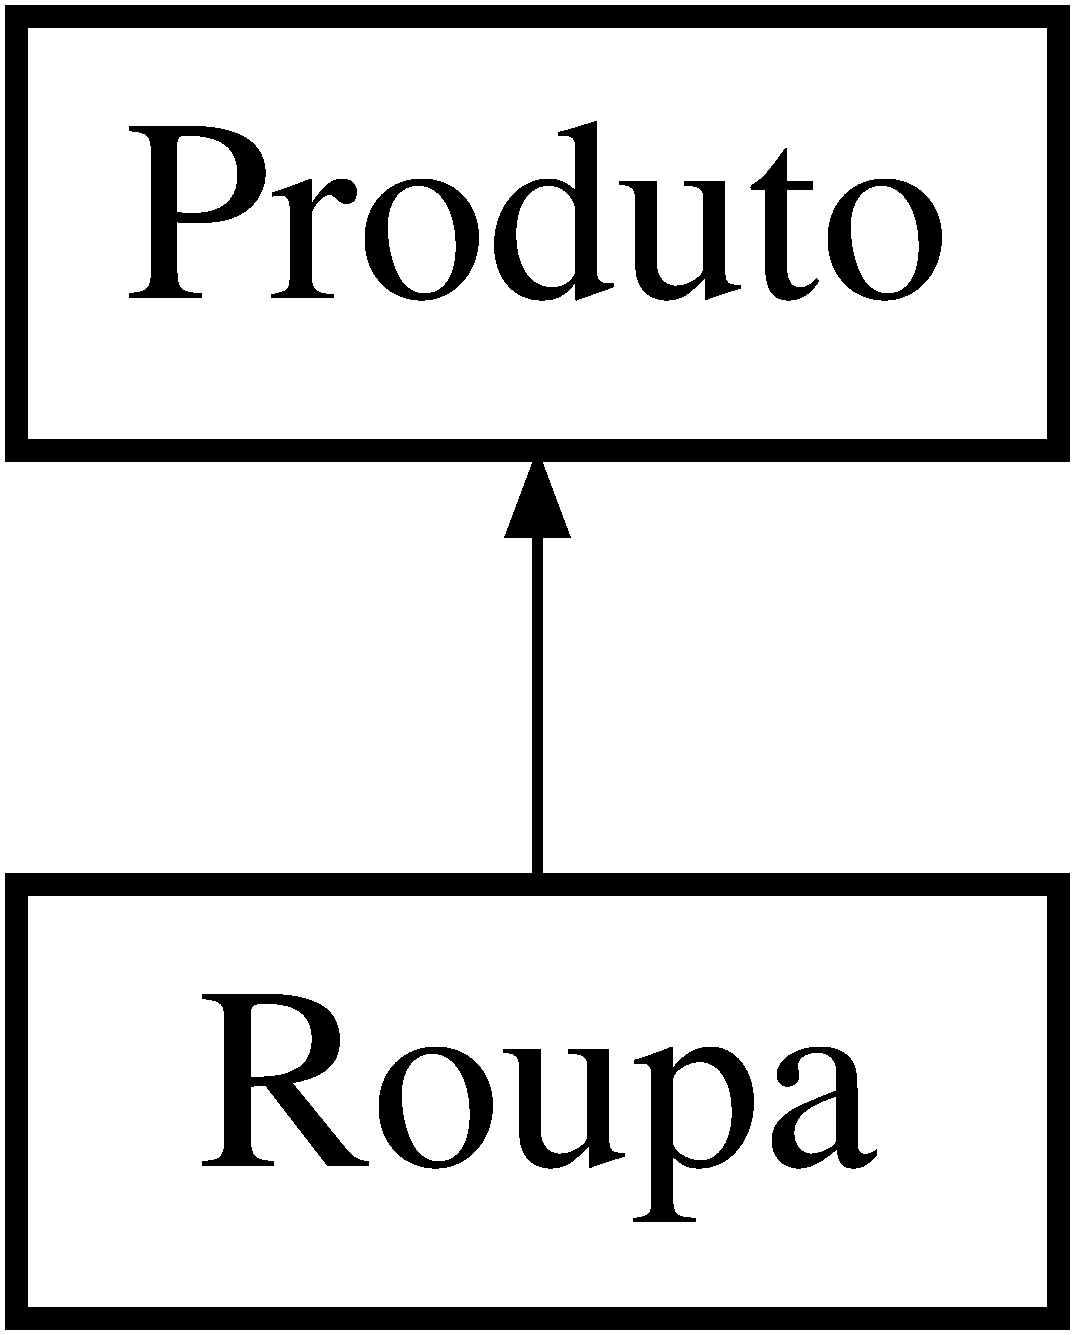
\includegraphics[height=2.000000cm]{d9/d53/classRoupa}
\end{center}
\end{figure}
\subsection*{Membros públicos}
\begin{DoxyCompactItemize}
\item 
\hypertarget{classRoupa_a0b8186c1c35089bebd88c8a3d0acf74b}{\hyperlink{classRoupa_a0b8186c1c35089bebd88c8a3d0acf74b}{Roupa} ()}\label{classRoupa_a0b8186c1c35089bebd88c8a3d0acf74b}

\begin{DoxyCompactList}\small\item\em Método construtor padrão de \hyperlink{classRoupa}{Roupa}. \end{DoxyCompactList}\item 
\hyperlink{classRoupa_aad1c967e981fd9605e0548432d035770}{Roupa} (int \hyperlink{classProduto_a76711f92305c825f07549734cd7c6ade}{tag}, string codigo\-Barra, string \hyperlink{classProduto_ab04a024e24feb7f79774e280356f6bc7}{descricao}, short \hyperlink{classProduto_a2ad13f91582fd70e878fc449c7b77171}{preco}, string marca, string sexo, string tamanho)
\begin{DoxyCompactList}\small\item\em Método construtor parametrizado de \hyperlink{classRoupa}{Roupa}. \end{DoxyCompactList}\item 
\hypertarget{classRoupa_af7d0589e854d5dfef94346856d417544}{\hyperlink{classRoupa_af7d0589e854d5dfef94346856d417544}{$\sim$\-Roupa} ()}\label{classRoupa_af7d0589e854d5dfef94346856d417544}

\begin{DoxyCompactList}\small\item\em Interface destrutor de \hyperlink{classProduto}{Produto} definida para \hyperlink{classRoupa}{Roupa}  Método virtual da classe \hyperlink{classProduto}{Produto} redefinida para um objeto \hyperlink{classRoupa}{Roupa}. \end{DoxyCompactList}\item 
string \hyperlink{classRoupa_a627cb05c4d7401b97bae9902b6fcbff8}{get\-Marca} ()
\begin{DoxyCompactList}\small\item\em Método de captura de marca. \end{DoxyCompactList}\item 
string \hyperlink{classRoupa_aa9048e6bf54153c4217e75666458f969}{get\-Sexo} ()
\begin{DoxyCompactList}\small\item\em Método de captura de sexo. \end{DoxyCompactList}\item 
string \hyperlink{classRoupa_add2ba0c5b5b10c0d99cd85363ce22960}{get\-Tamanho} ()
\begin{DoxyCompactList}\small\item\em Método de captura de tamanho. \end{DoxyCompactList}\item 
void \hyperlink{classRoupa_a7a5daab180f39dc0f6356f0a029b7174}{set\-Marca} (string marca)
\begin{DoxyCompactList}\small\item\em Método de atribuição de marca. \end{DoxyCompactList}\item 
void \hyperlink{classRoupa_a6cf689693ff15cb33cf258171ccd11db}{set\-Sexo} (string sexo)
\begin{DoxyCompactList}\small\item\em Método de atribuição de categoria sexo. \end{DoxyCompactList}\item 
void \hyperlink{classRoupa_a26a2f97971c92f32b9eb5b3c73d2d825}{set\-Tamanho} (string tamanho)
\begin{DoxyCompactList}\small\item\em Método de atribuição de tamanho. \end{DoxyCompactList}\end{DoxyCompactItemize}
\subsection*{Additional Inherited Members}


\subsection{Descrição detalhada}
Classe \hyperlink{classRoupa}{Roupa}, derivada de \hyperlink{classProduto}{Produto}. 

\subsection{Documentação dos Construtores \& Destrutor}
\hypertarget{classRoupa_aad1c967e981fd9605e0548432d035770}{\index{Roupa@{Roupa}!Roupa@{Roupa}}
\index{Roupa@{Roupa}!Roupa@{Roupa}}
\subsubsection[{Roupa}]{\setlength{\rightskip}{0pt plus 5cm}Roupa\-::\-Roupa (
\begin{DoxyParamCaption}
\item[{int}]{tag, }
\item[{string}]{codigo\-Barra, }
\item[{string}]{descricao, }
\item[{short}]{preco, }
\item[{string}]{marca, }
\item[{string}]{sexo, }
\item[{string}]{tamanho}
\end{DoxyParamCaption}
)}}\label{classRoupa_aad1c967e981fd9605e0548432d035770}


Método construtor parametrizado de \hyperlink{classRoupa}{Roupa}. 


\begin{DoxyParams}{Parâmetros}
{\em int} & tag -\/ categoria do \hyperlink{classProduto}{Produto} \\
\hline
{\em string} & codigo -\/ Codigo de barras do \hyperlink{classProduto}{Produto} \\
\hline
{\em string} & descricao -\/ Descrição do \hyperlink{classProduto}{Produto} \\
\hline
{\em short} & preco -\/ Preço do \hyperlink{classProduto}{Produto} \\
\hline
{\em string} & marca -\/ Recebe a marca da roupa \\
\hline
{\em string} & sexo -\/ Define a categoria da roupa em relação a sexo \\
\hline
{\em string} & tamanho -\/ Define o tamanho da roupa \\
\hline
\end{DoxyParams}


\subsection{Documentação dos métodos}
\hypertarget{classRoupa_a627cb05c4d7401b97bae9902b6fcbff8}{\index{Roupa@{Roupa}!get\-Marca@{get\-Marca}}
\index{get\-Marca@{get\-Marca}!Roupa@{Roupa}}
\subsubsection[{get\-Marca}]{\setlength{\rightskip}{0pt plus 5cm}std\-::string Roupa\-::get\-Marca (
\begin{DoxyParamCaption}
{}
\end{DoxyParamCaption}
)}}\label{classRoupa_a627cb05c4d7401b97bae9902b6fcbff8}


Método de captura de marca. 

\begin{DoxyReturn}{Retorna}
Retorna a marca do produto 
\end{DoxyReturn}
\hypertarget{classRoupa_aa9048e6bf54153c4217e75666458f969}{\index{Roupa@{Roupa}!get\-Sexo@{get\-Sexo}}
\index{get\-Sexo@{get\-Sexo}!Roupa@{Roupa}}
\subsubsection[{get\-Sexo}]{\setlength{\rightskip}{0pt plus 5cm}string Roupa\-::get\-Sexo (
\begin{DoxyParamCaption}
{}
\end{DoxyParamCaption}
)}}\label{classRoupa_aa9048e6bf54153c4217e75666458f969}


Método de captura de sexo. 

\begin{DoxyReturn}{Retorna}
Retorna a categoria sexo da \hyperlink{classRoupa}{Roupa} 
\end{DoxyReturn}
\hypertarget{classRoupa_add2ba0c5b5b10c0d99cd85363ce22960}{\index{Roupa@{Roupa}!get\-Tamanho@{get\-Tamanho}}
\index{get\-Tamanho@{get\-Tamanho}!Roupa@{Roupa}}
\subsubsection[{get\-Tamanho}]{\setlength{\rightskip}{0pt plus 5cm}string Roupa\-::get\-Tamanho (
\begin{DoxyParamCaption}
{}
\end{DoxyParamCaption}
)}}\label{classRoupa_add2ba0c5b5b10c0d99cd85363ce22960}


Método de captura de tamanho. 

\begin{DoxyReturn}{Retorna}
Retorna o tamanho da roupa 
\end{DoxyReturn}
\hypertarget{classRoupa_a7a5daab180f39dc0f6356f0a029b7174}{\index{Roupa@{Roupa}!set\-Marca@{set\-Marca}}
\index{set\-Marca@{set\-Marca}!Roupa@{Roupa}}
\subsubsection[{set\-Marca}]{\setlength{\rightskip}{0pt plus 5cm}void Roupa\-::set\-Marca (
\begin{DoxyParamCaption}
\item[{string}]{marca}
\end{DoxyParamCaption}
)}}\label{classRoupa_a7a5daab180f39dc0f6356f0a029b7174}


Método de atribuição de marca. 


\begin{DoxyParams}{Parâmetros}
{\em Recebe} & string marca \\
\hline
\end{DoxyParams}
\hypertarget{classRoupa_a6cf689693ff15cb33cf258171ccd11db}{\index{Roupa@{Roupa}!set\-Sexo@{set\-Sexo}}
\index{set\-Sexo@{set\-Sexo}!Roupa@{Roupa}}
\subsubsection[{set\-Sexo}]{\setlength{\rightskip}{0pt plus 5cm}void Roupa\-::set\-Sexo (
\begin{DoxyParamCaption}
\item[{string}]{sexo}
\end{DoxyParamCaption}
)}}\label{classRoupa_a6cf689693ff15cb33cf258171ccd11db}


Método de atribuição de categoria sexo. 


\begin{DoxyParams}{Parâmetros}
{\em Recebe} & string sexo \\
\hline
\end{DoxyParams}
\hypertarget{classRoupa_a26a2f97971c92f32b9eb5b3c73d2d825}{\index{Roupa@{Roupa}!set\-Tamanho@{set\-Tamanho}}
\index{set\-Tamanho@{set\-Tamanho}!Roupa@{Roupa}}
\subsubsection[{set\-Tamanho}]{\setlength{\rightskip}{0pt plus 5cm}void Roupa\-::set\-Tamanho (
\begin{DoxyParamCaption}
\item[{string}]{tamanho}
\end{DoxyParamCaption}
)}}\label{classRoupa_a26a2f97971c92f32b9eb5b3c73d2d825}


Método de atribuição de tamanho. 


\begin{DoxyParams}{Parâmetros}
{\em Recebe} & string tamanho \\
\hline
\end{DoxyParams}


A documentação para esta classe foi gerada a partir dos seguintes ficheiros\-:\begin{DoxyCompactItemize}
\item 
include/roupa.\-h\item 
src/\hyperlink{roupa_8cpp}{roupa.\-cpp}\end{DoxyCompactItemize}

\chapter{Documentação do ficheiro}
\hypertarget{bebida_8h}{\section{Referência ao ficheiro include/bebida.h}
\label{bebida_8h}\index{include/bebida.\-h@{include/bebida.\-h}}
}


Definição da classe \hyperlink{classBebida}{Bebida} em C++.  


{\ttfamily \#include \char`\"{}produto.\-h\char`\"{}}\\*
\subsection*{Componentes}
\begin{DoxyCompactItemize}
\item 
class \hyperlink{classBebida}{Bebida}
\begin{DoxyCompactList}\small\item\em Classe \hyperlink{classBebida}{Bebida}, derivada de \hyperlink{classProduto}{Produto}. \end{DoxyCompactList}\end{DoxyCompactItemize}


\subsection{Descrição detalhada}
Definição da classe \hyperlink{classBebida}{Bebida} em C++. \begin{DoxyAuthor}{Autor}
Bruno César L. Silva 
\end{DoxyAuthor}
\begin{DoxySince}{Desde}
10/05/2018 
\end{DoxySince}
\begin{DoxyDate}{Data}
14/05/2018 
\end{DoxyDate}

\hypertarget{fruta_8h}{\section{Referência ao ficheiro include/fruta.h}
\label{fruta_8h}\index{include/fruta.\-h@{include/fruta.\-h}}
}


Definição da classe \hyperlink{classFruta}{Fruta} em C++.  


{\ttfamily \#include \char`\"{}produto.\-h\char`\"{}}\\*
\subsection*{Componentes}
\begin{DoxyCompactItemize}
\item 
class \hyperlink{classFruta}{Fruta}
\begin{DoxyCompactList}\small\item\em Classe \hyperlink{classFruta}{Fruta}, derivada de \hyperlink{classProduto}{Produto}. \end{DoxyCompactList}\end{DoxyCompactItemize}


\subsection{Descrição detalhada}
Definição da classe \hyperlink{classFruta}{Fruta} em C++. \begin{DoxyAuthor}{Autor}
Bruno César L. Silva 
\end{DoxyAuthor}
\begin{DoxySince}{Desde}
10/05/2018 
\end{DoxySince}
\begin{DoxyDate}{Data}
14/05/2018 
\end{DoxyDate}

\hypertarget{produto_8h}{\section{Referência ao ficheiro include/produto.h}
\label{produto_8h}\index{include/produto.\-h@{include/produto.\-h}}
}


Definição da classe \hyperlink{classProduto}{Produto} em C++.  


{\ttfamily \#include $<$iostream$>$}\\*
\subsection*{Componentes}
\begin{DoxyCompactItemize}
\item 
class \hyperlink{classProduto}{Produto}
\end{DoxyCompactItemize}


\subsection{Descrição detalhada}
Definição da classe \hyperlink{classProduto}{Produto} em C++. \begin{DoxyAuthor}{Autor}
Bruno César L. Silva 
\end{DoxyAuthor}
\begin{DoxySince}{Desde}
10/05/2018 
\end{DoxySince}
\begin{DoxyDate}{Data}
14/05/2018 
\end{DoxyDate}

\hypertarget{bebida_8cpp}{\section{Referência ao ficheiro src/bebida.cpp}
\label{bebida_8cpp}\index{src/bebida.\-cpp@{src/bebida.\-cpp}}
}


Implementação da classe \hyperlink{classBebida}{Bebida} em C++.  


{\ttfamily \#include $<$iomanip$>$}\\*
{\ttfamily \#include $<$istream$>$}\\*
{\ttfamily \#include $<$sstream$>$}\\*
{\ttfamily \#include \char`\"{}bebida.\-h\char`\"{}}\\*


\subsection{Descrição detalhada}
Implementação da classe \hyperlink{classBebida}{Bebida} em C++. \begin{DoxyAuthor}{Autor}
Bruno César L. Silva 
\end{DoxyAuthor}
\begin{DoxySince}{Desde}
10/05/2018 
\end{DoxySince}
\begin{DoxyDate}{Data}
14/05/2018
\end{DoxyDate}
\hypertarget{roupa_8cpp_DESCRIÇÃO}{}\subsection{D\-E\-S\-C\-R\-IÇÃ\-O}\label{roupa_8cpp_DESCRIÇÃO}
Implementa a classe \hyperlink{classBebida}{Bebida}, derivada da classe \hyperlink{classProduto}{Produto}. 
\hypertarget{fruta_8cpp}{\section{Referência ao ficheiro src/fruta.cpp}
\label{fruta_8cpp}\index{src/fruta.\-cpp@{src/fruta.\-cpp}}
}


Implementação da classe \hyperlink{classFruta}{Fruta} em C++.  


{\ttfamily \#include $<$iomanip$>$}\\*
{\ttfamily \#include \char`\"{}fruta.\-h\char`\"{}}\\*


\subsection{Descrição detalhada}
Implementação da classe \hyperlink{classFruta}{Fruta} em C++. \begin{DoxyAuthor}{Autor}
Bruno César L. Silva 
\end{DoxyAuthor}
\begin{DoxySince}{Desde}
10/05/2018 
\end{DoxySince}
\begin{DoxyDate}{Data}
14/05/2018
\end{DoxyDate}
\hypertarget{roupa_8cpp_DESCRIÇÃO}{}\subsection{D\-E\-S\-C\-R\-IÇÃ\-O}\label{roupa_8cpp_DESCRIÇÃO}
Implementa a classe \hyperlink{classFruta}{Fruta}, derivada da classe \hyperlink{classProduto}{Produto}. 
\hypertarget{produto_8cpp}{\section{Referência ao ficheiro src/produto.cpp}
\label{produto_8cpp}\index{src/produto.\-cpp@{src/produto.\-cpp}}
}


Implementação da classe \hyperlink{classProduto}{Produto} em C++.  


{\ttfamily \#include $<$iostream$>$}\\*
{\ttfamily \#include \char`\"{}produto.\-h\char`\"{}}\\*
\subsection*{Funções}
\begin{DoxyCompactItemize}
\item 
double \hyperlink{produto_8cpp_a13cc75bc264a9557efef0353b184d3e4}{operator+} (\hyperlink{classProduto}{Produto} \&a, \hyperlink{classProduto}{Produto} \&b)
\item 
double \hyperlink{produto_8cpp_af98881fb5c5587f7372a27edbe6bd808}{operator-\/} (\hyperlink{classProduto}{Produto} \&a, \hyperlink{classProduto}{Produto} \&b)
\item 
bool \hyperlink{produto_8cpp_adf4b96b0581708b8aa8bb2932bac578a}{operator==} (\hyperlink{classProduto}{Produto} \&a, \hyperlink{classProduto}{Produto} \&b)
\item 
std\-::ostream \& \hyperlink{produto_8cpp_a3f8bbab15d5b8943ac04af1bc6eec1bf}{operator$<$$<$} (std\-::ostream \&o, \hyperlink{classProduto}{Produto} const \&p)
\end{DoxyCompactItemize}


\subsection{Descrição detalhada}
Implementação da classe \hyperlink{classProduto}{Produto} em C++. \begin{DoxyAuthor}{Autor}
Bruno César L. Silva 
\end{DoxyAuthor}
\begin{DoxySince}{Desde}
10/05/2018 
\end{DoxySince}
\begin{DoxyDate}{Data}
14/05/2018
\end{DoxyDate}
\hypertarget{roupa_8cpp_DESCRIÇÃO}{}\subsection{D\-E\-S\-C\-R\-IÇÃ\-O}\label{roupa_8cpp_DESCRIÇÃO}
Implementa a classe \hyperlink{classProduto}{Produto} genêrica, base para todos os produtos da aplicação. 

\subsection{Documentação das funções}
\hypertarget{produto_8cpp_a13cc75bc264a9557efef0353b184d3e4}{\index{produto.\-cpp@{produto.\-cpp}!operator+@{operator+}}
\index{operator+@{operator+}!produto.cpp@{produto.\-cpp}}
\subsubsection[{operator+}]{\setlength{\rightskip}{0pt plus 5cm}double operator+ (
\begin{DoxyParamCaption}
\item[{{\bf Produto} \&}]{a, }
\item[{{\bf Produto} \&}]{b}
\end{DoxyParamCaption}
)}}\label{produto_8cpp_a13cc75bc264a9557efef0353b184d3e4}

\begin{DoxyParams}{Parâmetros}
{\em \hyperlink{classProduto}{Produto}} & \&a instância de \hyperlink{classProduto}{Produto} \\
\hline
{\em \hyperlink{classProduto}{Produto}} & \&b instância de \hyperlink{classProduto}{Produto} \\
\hline
\end{DoxyParams}
\begin{DoxyReturn}{Retorna}
retorna um double resultado da soma dos preços de dois Produtos 
\end{DoxyReturn}
\hypertarget{produto_8cpp_af98881fb5c5587f7372a27edbe6bd808}{\index{produto.\-cpp@{produto.\-cpp}!operator-\/@{operator-\/}}
\index{operator-\/@{operator-\/}!produto.cpp@{produto.\-cpp}}
\subsubsection[{operator-\/}]{\setlength{\rightskip}{0pt plus 5cm}double operator-\/ (
\begin{DoxyParamCaption}
\item[{{\bf Produto} \&}]{a, }
\item[{{\bf Produto} \&}]{b}
\end{DoxyParamCaption}
)}}\label{produto_8cpp_af98881fb5c5587f7372a27edbe6bd808}

\begin{DoxyParams}{Parâmetros}
{\em \hyperlink{classProduto}{Produto}} & \&a instância de \hyperlink{classProduto}{Produto} \\
\hline
{\em \hyperlink{classProduto}{Produto}} & \&b instância de \hyperlink{classProduto}{Produto} \\
\hline
\end{DoxyParams}
\begin{DoxyReturn}{Retorna}
retorna um double resultado da subtração dos preços de dois Produtos 
\end{DoxyReturn}
\hypertarget{produto_8cpp_a3f8bbab15d5b8943ac04af1bc6eec1bf}{\index{produto.\-cpp@{produto.\-cpp}!operator$<$$<$@{operator$<$$<$}}
\index{operator$<$$<$@{operator$<$$<$}!produto.cpp@{produto.\-cpp}}
\subsubsection[{operator$<$$<$}]{\setlength{\rightskip}{0pt plus 5cm}std\-::ostream\& operator$<$$<$ (
\begin{DoxyParamCaption}
\item[{std\-::ostream \&}]{o, }
\item[{{\bf Produto} const \&}]{p}
\end{DoxyParamCaption}
)}}\label{produto_8cpp_a3f8bbab15d5b8943ac04af1bc6eec1bf}

\begin{DoxyParams}{Parâmetros}
{\em ostream} & \&o operador de inserção \\
\hline
{\em \hyperlink{classProduto}{Produto}} & t uma instância de produto \\
\hline
\end{DoxyParams}
\begin{DoxyReturn}{Retorna}
retorna a instância do operador de inserção 
\end{DoxyReturn}
\hypertarget{produto_8cpp_adf4b96b0581708b8aa8bb2932bac578a}{\index{produto.\-cpp@{produto.\-cpp}!operator==@{operator==}}
\index{operator==@{operator==}!produto.cpp@{produto.\-cpp}}
\subsubsection[{operator==}]{\setlength{\rightskip}{0pt plus 5cm}bool operator== (
\begin{DoxyParamCaption}
\item[{{\bf Produto} \&}]{a, }
\item[{{\bf Produto} \&}]{b}
\end{DoxyParamCaption}
)}}\label{produto_8cpp_adf4b96b0581708b8aa8bb2932bac578a}

\begin{DoxyParams}{Parâmetros}
{\em \hyperlink{classProduto}{Produto}} & \&a instância de \hyperlink{classProduto}{Produto} \\
\hline
{\em \hyperlink{classProduto}{Produto}} & \&b instância de \hyperlink{classProduto}{Produto} \\
\hline
\end{DoxyParams}
\begin{DoxyReturn}{Retorna}
Se os códigos de barras forem iguais retorna true, se não, falso 
\end{DoxyReturn}

\hypertarget{roupa_8cpp}{\section{Referência ao ficheiro src/roupa.cpp}
\label{roupa_8cpp}\index{src/roupa.\-cpp@{src/roupa.\-cpp}}
}


Implementação da classe \hyperlink{classRoupa}{Roupa} em C++.  


{\ttfamily \#include $<$iomanip$>$}\\*
{\ttfamily \#include \char`\"{}roupa.\-h\char`\"{}}\\*


\subsection{Descrição detalhada}
Implementação da classe \hyperlink{classRoupa}{Roupa} em C++. \begin{DoxyAuthor}{Autor}
Bruno César L. Silva 
\end{DoxyAuthor}
\begin{DoxySince}{Desde}
10/05/2018 
\end{DoxySince}
\begin{DoxyDate}{Data}
14/05/2018
\end{DoxyDate}
\hypertarget{roupa_8cpp_DESCRIÇÃO}{}\subsection{D\-E\-S\-C\-R\-IÇÃ\-O}\label{roupa_8cpp_DESCRIÇÃO}
Implementa a classe \hyperlink{classRoupa}{Roupa}, derivada da classe \hyperlink{classProduto}{Produto}. 
%--- End generated contents ---

% Index
\newpage
\phantomsection
\addcontentsline{toc}{chapter}{Índice}
\printindex

\end{document}
